\chapter{Teknologi}
I dette afsnit undersøges Ultralyds Robotarmen ud fra et teknologisk perspektiv. Afsnittet er blandt andet baseret på besøg hos Hospitalsenheden Horsens og Hospitalsenhed Midt i Viborg. Den teknologiske løsning består af:
\begin{itemize}
\item UR3 Robotarm fra Universal Robots incl. software til styring af denne
\item Stativ til robotten
\item Joystick
\item Computer
\item Holder til ultralydsprobe
\end{itemize}
Denne løsning skal kobles til det allerede eksisterende udstyr. Derfor er produktet en add-on løsning, hvilket betyder at produktet skal købes udover det almindelige scanningsudstyr. Det nuværende system består af Voluson S6 inkl. DICOM og printer, samt diverse ultralydsprober.  

%Se bilag økonomi. 
\begin{figure}[H]
	\begin{minipage}{0.45\textwidth}
		\centering
		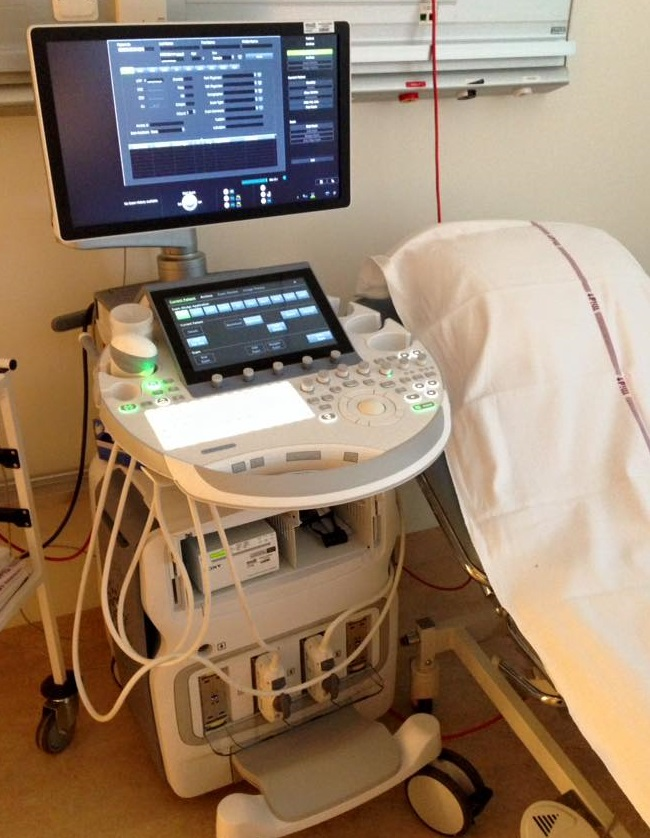
\includegraphics[width=\textwidth]{Figurer/udstyrHorsens.jpg}
		\caption{Nuværende udstyr: Voluson S6 med tilbehør. Billede fra Hospitalsenhed Horsens.}
		\label{udstyrHorsens}
	\end{minipage}
	\hspace{0.02\textwidth}
	\begin{minipage}{0.55\textwidth}
		\centering
		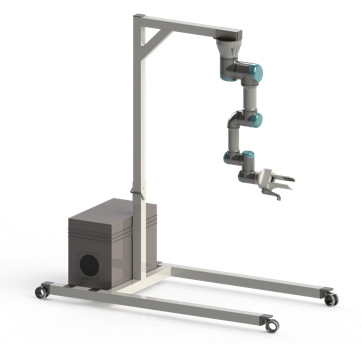
\includegraphics[width=\textwidth]{Figurer/StativMedUR3Render.png}
		\caption{Animation af robotarmen på stativet.}
		\label{Robotstativ}
	\end{minipage}
\end{figure}

\section{Anvendelsesområde}
Produktet skal anvendes til ultralydsscanninger af gravide borgere. Robotarmen er fastmonteret på et stativ, så den hænger over den gravide. Det medvirker en større trykkraft, end hvis den stod på gulvet. For at skabe mobilitet, er stativet placeret på hjul. Hjulene kan låses for af sikkerhedsmæssige årsager og for en statisk placering i forhold til den gravide. På robotarmen findes en universalholder til ultralydsproben. Holderen er universal og passer til alle større fabrikanters håndholdte ultralydsprober, bortset fra vagnialprober.\\

Stativet med robotarmen skal være på den modsatte side af sengen, end sonografen. Dette sikre sonografens udsyn og nærkontakt til den gravide.
Robotarmen skal holde ultralydsproben over den gravide, mens robotarmen styres af sonografen via et joystick. Derved undgår sonografen fysisk akavede arbejdsstillinger. \\
Joysticket har en dummy-probe, som ikke har nogle probe egenskaber, men den skal give sonografen en følelse af at sidde med en ægte probe i hånden.
Systemet skal kunne overføre det tryk, som sonografen påvirker joysticket med, til robotarmen.
%Hvis sonografen påvirker joysticket med en kræft større end 15 N, (skal lige tjekkes med Søren) slår robotarmen automatisk fra, af sikkerhedsmæssige grunde. 

\begin{figure}[H]\centering
	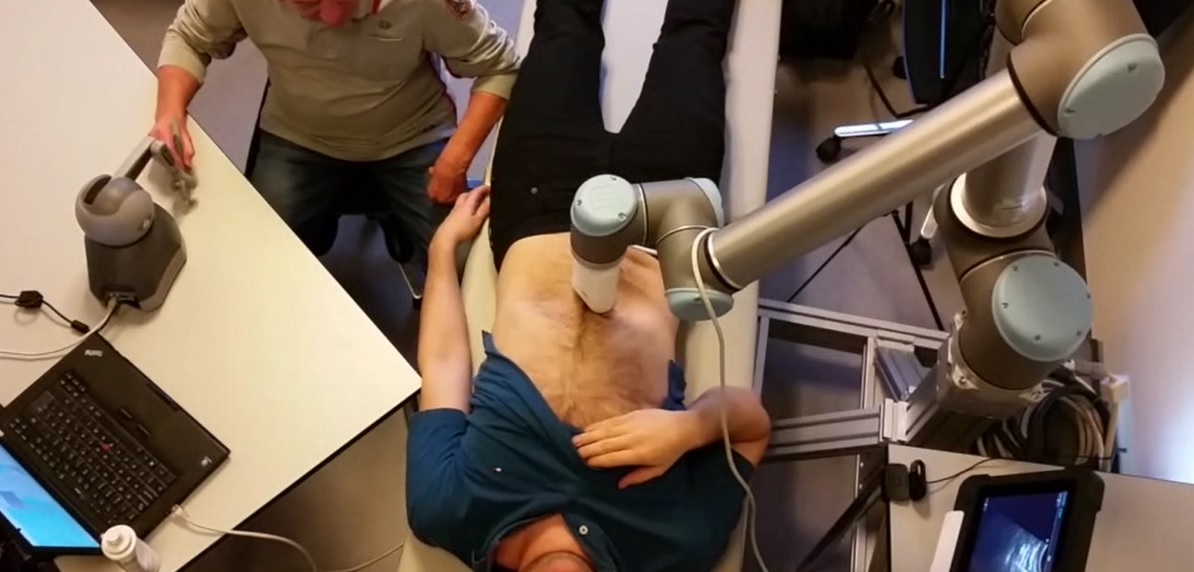
\includegraphics[width = 1.0\textwidth]{Figurer/ergonomiskLosning.jpg}
	\caption{Eksempel på opstilling af Ultralyds Robotarm. Nu er robotarmen placeret over borgeren og ikke ved side af. På billedet ses joystick(tv.) og robotarm(th.).  }
	\label{ergonomiskLosning}
\end{figure}

\section{Specifikationer}
Robotarmeren har en rækkevide på 50 cm, hvilket angiver hvor langt den kan række ud, som var det en arm. Den vejer 11 kg, derfor skal stativet være bygget dertil. Robotarmen har 6-graders frihed, som betyder at den kan bevæge sig i x-, y- og z-aksens retning og med drejevirkning om hver akse, samtidigt kan den lave en +/- 360 graders rotation. \\
(Skulder og base led kan dreje med en hastighed på 360grader/sekund,  andre led har en hastighed på 180grader/sekund.). \\
Robotarmen kræver en 100-240 VAC, 50-60Hz strømforsyning, som betyder at den kom blive sat til en almindelig dansk stikkontakt. 
\newline 
Joysticket har bevægelighed som et håndled, derved har den også de begrænsninger som findes ved et håndled. Det har 6-graders frihed, så det passer med robotarmen. Se bilag UR3 Tekniske specifikationer. \\

Der medfølger software til robotarmen, som både er koblingslinket mellem joystick og robotarm og styring deraf. Det er her bevægelserne fra joysticket omsættes til robotarmens bevægelser. Det er også her flere sikkerhedsmæssige foranstaltninger er placeret. Nogle indbygget i robotarmen, for eksempel stopper den øjeblikligt, hvis den bliver mødt med kraft på 50 N, det er blandt andet derfor den må benyttes på et hospital.    

\section{Effektivitet}
Ultralyds Robotarmen vil blive benyttet til 70-80\% af scannningerne på de gravide, da de sidste 20-30\% af scanningerne er for komplicerede til at robotten kan udføre dem. Derfor skal sonografen manuelt foretage de sidste 20-30\% af scanningerne på den nuværende metode. \\ 
De komplicerede ultralydsscanninger er blandt andet scanninger på kvinder med højt BMI eller kvinder med bagoverbøjet livmoder. Dette er ud fra antagelser fra CEO Søren Pallesen af Robotic Ultrasound ApS. 
\newline 
Ultralyds Robotarmen har ikke indflydelse på billedekvalitet eller kvaliteten af selve scanningen. Dette kommer af at ultralydsproperne er de samme, som man før har benyttet. \\Computeren i Voluson S6 indeholder det samme software til billedanalyse og til diverse instrumenter som bruges under scanninger. Det er blandet andet tale om software til vækst- og flowmålinger af fostre.   \\
Når sonografen vil trykke med ultralyds proben på den gravide borger, vil trykkraften bliver overført til joysticket og dummy-proben så sonografen får den korrekte tryk feedback. Derved vil sonografen have følelsen af, at der bliver trykket direkte på borgeren og kan dermed bedre selv have føling med situationen. 
\section{Sikkerhed}
I softwaren til styring fra joystick til robotarm findes en sikkerhedsindstilling, hvor en grænse for trykpåvirkningen skal indstilles. Hvis der af menneskelige eller teknologisk fejl bliver påvirket med en kraft over grænsen, vil robotarmen automatisk slå fra og stoppe. \\
Som tidligere nævnt er der også en sikkerhed i at robotarmen stopper sine bevægelser hvis den bliver ramt af en kraft på over 5 N. Den foranstaltning gør at den ikke vil gøre skade på mennesker eller genstande ved at ramme dem. 

\section{Delkonklusion}
Ultralyds robotarmen kommer kun til at udføre 70-80\% af scanningerne, hvilket gør at sonograferne stadig skal udføre nogle af scanningerne manuelt. Men at robotarmen kan udføre størstedelen af scanningerne gør, at en stor del af belastningen på sonograferne fjernes. Derfor kan de mest komplicerede scanninger udføres manuelt, da sonograferne vil have mere styrke til disse.\\

Der er tidliger blevet testet med robotarme i forbindelse med ultralydsscaninger, her dog på hjertet. Her viste det sig ikke at være et problem at styre selve armen.  Denne undersøgelse ligger nogle år tilbage i tiden og derfor at teknologien allerede ændret sig meget. Derfor menes det ikke at styringe, betjening og implementering af ultralyds robotarmen til scanninger af gravide ikke vil give de store problemer i sig selv. Der vil naturligvis altid være en overgangsperiode, hvor sonograferne skal vænne sig til at benytte joysticket. 